\documentclass{nature3}
\usepackage{graphicx}
\usepackage{float}
\usepackage{verbatim}
\usepackage{hyperref}
\usepackage{amsmath}
\usepackage{amssymb}
\usepackage{aas_macros_nature}
\usepackage{lineno}
\usepackage{caption}
\usepackage{rotating} % sidewaystable

\linespread{1.0}
\linenumbers % turn line numbering on or off

\newcommand{\farcm}{\mbox{\ensuremath{.\mkern-4mu^\prime}}}%    % fractional arcminute symbol: 0.'0
\newcommand{\farcs}{\mbox{\ensuremath{.\!\!^{\prime\prime}}}}%  % fractional arcsecond symbol: 0.''0

\newcommand{\kms}{\ensuremath{\rm km\,s^{-1}}}
\newcommand{\ms}{\ensuremath{\rm m\,s^{-1}}}

\renewcommand*{\thefootnote}{\fnsymbol{footnote}}

%%%%%%%%%%%%%%%%
% INSTITUTIONS %
%%%%%%%%%%%%%%%%
\newcommand{\carnegie}{Observatories of the Carnegie Institution for Science, Pasadena, CA 91101, USA}
\newcommand{\caltech}{Department of Astronomy, California Institute of Technology, Pasadena, CA 91125, USA}
%%%%%%%%%%%%%%%%

%%%%%%%%%%
% VALUES %
%%%%%%%%%%
% NOTE: might need to be ingested before submission 
\newcommand{\stteff}{YYYY}
\newcommand{\stagemyr}{40}
\newcommand{\periodhr}{3.930}


%%%%%%%%%%%%%%%%%%%%%%%%%%%%%%%%%%%%%%%%%%
%%%%%%%%%%%%%%%%%%%%%%%%%%%%%%%%%%%%%%%%%%

\title{A Plasma Torus Around a Young Low-Mass Star}

\begin{document}

\author{Luke G. Bouma$^{1,2}$}

\maketitle

\scriptsize
\begin{affiliations}
\item \carnegie
\item \caltech
\item Carnegie Fellow; 51 Pegasi b Fellow
\end{affiliations}
\normalsize

%%%%%%%%%%%%%%%%%%%%%%%%%%%%%%%%%%%%%%%%%%%%%%%%%%%%%%%%%%%%%%%%%%%%%%%%%%%%%%%
%%%%%%%%%%%%%%%%%%%%%%%%%%%%%%%%%%%%%%%%%%%%%%%%%%%%%%%%%%%%%%%%%%%%%%%%%%%%%%%

\begin{abstract}
\normalfont
Roughly one percent of red dwarfs younger than 100 million years show
structured, periodic optical light curves suggestive of transiting
opaque material that corotates with the star
\cite{Rebull2016,Stauffer2017,Rebull2018,Bouma2024}.  However, the
composition, origin, and even the existence of this material are
uncertain. The main alternative hypothesis is that these complex
periodic variables (CPVs) are explained by complex distributions of
bright or dark regions on the stellar surfaces \cite{Koen2021}.
Here, we present time-series spectroscopy and photometry of a
rapidly-rotating ($P$=3.9\,hr) CPV, TIC~141146667. The spectra show
sinusoidal time-varying Balmer emission at twice to four times the
star's equatorial velocity, directly demonstrating for the first
time the existence of corotating clumps of circumstellar plasma around a CPV.
Given that cool ($10^4$ K) plasma can persist in the hot ($10^6$ K)
coronae of rapidly-rotating stars with a wide range of masses
\cite{CollierCameron1989,Townsend2005,Dunstone2006,Petit2013,Waugh2022,Daley-Yates2024},
these data support the idea that the magnetospheres of the
lowest-mass stars can support long-lived, optically thick
clumps of material that explain the sharp photometric features seen in
CPVs.  The origin of this optically thick material and its
microphysical opacity remain unclear.
\end{abstract}

\maketitle

%%%%%%%%%%%%%%%%%%%%%%%%%%%%%%%%%%%%%%%%%%%%%%%%%%%%%%%%%%%%%%%%%%%%%%%%%%%%%%%
%%%%%%%%%%%%%%%%%%%%%%%%%%%%%%%%%%%%%%%%%%%%%%%%%%%%%%%%%%%%%%%%%%%%%%%%%%%%%%%

% Main text – up to 3,000 words, excluding abstract, Methods,
% references and figure legends.

\section{Main}
\label{sec:main}

M dwarfs, stars with masses below about half that of the Sun, are the
only type of star to offer near-term prospects for detecting the
atmospheres of rocky exoplanets with surface water \cite{NAP26141}.
Community investment with JWST has proceeded accordingly
\cite{Redfield2024,TRAPPIST1JWSTCommunityInitiative2024}.  How an M
dwarf's evolution influences its planets---especially the retention of
their atmospheres--- has in turn become a major theme in
exoplanet and stellar astrophysics.  Previous work has established
that most M dwarfs host close-in planets \cite{Dressing2015} that 
on average are subject to long circumstellar disk lifetimes
\cite{Ribas2015}, to high doses of UV radiation \cite{France2016},
and to a high incidence of flares and coronal mass ejections
\cite{Gunther2020}.  However, despite extensive work in these areas,
the plasma and magnetospheric environments that bathe young, close-in
exoplanets remain challenging to quantify.
Understanding these environments is crucial because they directly
impact atmospheric retention and habitability of close-in planets.

One glaring example of our current ignorance is the complex periodic
variables (CPVs).  While Figure~\ref{fig:lc} highlights the main
object of interest in this article, over one hundred analogous objects
have now been found by K2 and TESS
\cite{Rebull2016,Stauffer2017,Rebull2018,Zhan2019,Rebull2020,Bouma2024}.
These CPVs are phenomenologically identified based on their
structured, periodic optical light curves; most are M dwarfs with
rotation periods shorter than two days.  Within current sensitivity
limits, none host disks \cite{Stauffer2017,Bouma2024}.
However, $\approx$3\% of stars a few million years old show this complex
photometric behavior, an observed fraction which decreases to $\approx$0.3\% by
$\approx$150\,Myr \cite{Rebull2020}.
CPVs are a known source of astrophysical false positives in searches for
transiting exoplanets around young M dwarfs
\cite{vanEyken2012,Johns-Krull2016,Bouma2020}.

The two leading hypotheses for explaining CPVs are either that
transiting clumps of circumstellar material corotate with the star
\cite{Stauffer2017,Gunther2022,Bouma2024}, or that these stars
represent an extreme in naturally-occurring distributions of starspots
or faculae \cite{Koen2021}.  The main argument against a starspot-only
explanation invokes the timescales and amplitudes of the sharpest
photometric features.  However, no independent evidence has yet been
acquired for the presence of any circumstellar material.
Geometrically, transiting clumps would imply an occurrence a few to at
most ten times the observed rate.  The clumps could therefore exist
around 10-30\% of M dwarfs during their early lives.


\begin{figure}[!t]
  \centering
  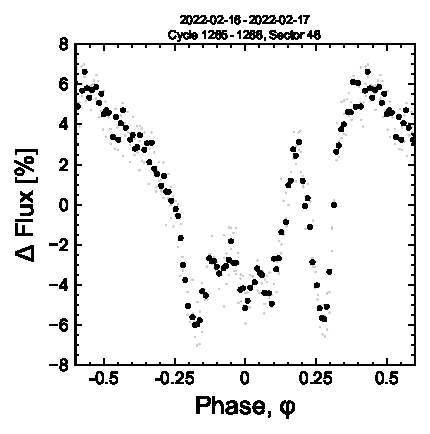
\includegraphics[width=0.7\textwidth]{figures/f1.pdf}
  \captionsetup{labelformat=empty}
  \caption{{\bf Figure 1 (Movie):  TIC~141146667 is a complex periodic
  variable (CPV).}  The online movie,
  \href{https://lgbouma.com/movies/TIC141146667_20250116.mp4}{available here},
  covers a baseline of 5{,}784 cycles irregularly sampled over three
  years.  The TESS light curve is phased to the \periodhr\ hour period
  in groups of three cycles per frame.  This is the period both of
  stellar rotation, and (we hypothesize) of corotating clumps of
  circumstellar material.  Raw data acquired with two minute sampling
  are in gray; black averages to 100 points per cycle.  Similar to
  other stars of this class, the sharp photometric features persist
  for tens to thousands of rotational cycles. }
  \label{fig:lc}
\end{figure}

The dearth of evidence for circumstellar material around CPVs is
surprising given that separate studies of young stars have, for
decades, reported that stellar coronae contain both hot ($10^6$ K) and
cool ($10^4$ K) plasma. In particular, time-series spectroscopy of stars
with a wide range of masses has shown periodic high-velocity
absorption and emission in Balmer lines such as H$\alpha$, interpreted
as long-lived, corotating clumps of cool plasma
\cite{CollierCameron1989,CollierCameron1992,Barnes2000,Donati2000,Dunstone2006,Skelly2008,Leitzinger2016,Cang2021}.
Such clumps are thought to be forced into corotation by the magnetic
field, and the exact geometry of where the plasma can accumulate is
dictated by the field's topology.  For instance, a magnetic dipole field
tilted with respect to the stellar spin axis
yields accumulations in a warped torus geometry
\cite{Townsend2005}, whereas in the limit of a single strong field
line, accumulation occurs at the line's apex, furthest from the star
\cite{Waugh2022}.  To date, none of these spectroscopic variables have
shown any photometric anomalies \cite{Bouma2024}, leaving open the
issue of whether they are related to CPVs.


In this study, we present the first spectroscopic detection of
corotating clumps of cool plasma around a CPV.  We identified
TIC~141146667 in previous work \cite{Bouma2024} by searching the TESS
two-minute data \cite{Ricker2015} for stars showing highly structured,
periodic light curves.  We selected the star for spectroscopy because
its brightness and rotation rate enabled an efficient search for 
variability in its line profiles.  We observed the star for five hours on
17~February~2024 (UT) using the High Resolution Echelle Spectrometer
(HIRES \cite{vogt_hires_1994}) on the 10\,m Keck I telescope.  TESS
observed the star over a four week interval from 30~January~2024 to
26~February~2024 with a duty cycle of 77\%.  During the HIRES
observations, scattered light from the Earth caused a gap in the TESS
photometry; TESS data collection resumed 12 hours (three rotation
cycles) after the spectra were acquired.  Extended Data
Figure~\ref{fig:fulllc} shows the detailed photometric behavior of the
star near the epoch of observation; the general photometric morphology
is similar before and after the data gap.


\section{Results}

\begin{figure}[!tp]
  \centering
  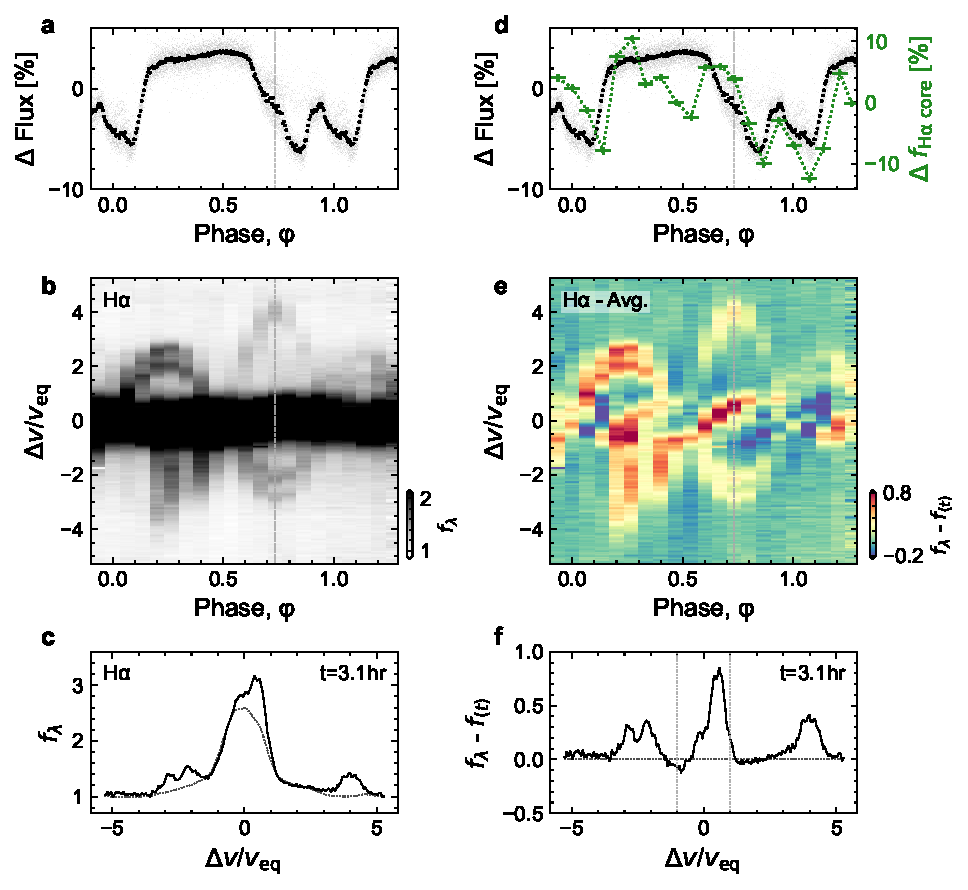
\includegraphics[width=0.99\textwidth]{figures/f2.pdf}
  \captionsetup{labelformat=empty}
  \caption{{\bf Figure 2 (Movie):}  
  Emission from circumstellar plasma orbiting TIC 141146667.
  The online movie,
  \href{https://lgbouma.com/movies/TIC141146667_sixpanel.mp4}{available here},
  shows the spectral evolution over five hours.
  {\bf a,} Average TESS light curve from 5 February 2024 to 26
  February 2024 folded on the \periodhr\ hour period.  Black
  points are phase-averaged; gray are the raw data.
  {\bf b,} Keck/HIRES H$\alpha$ spectra acquired on 17
  February 2024.  The continuum is set to unity, and the darkest color
  is at twice the continuum to accentuate emission outside the line
  core ($|v/v_{\rm eq}|>1$, for $v_{\rm eq}$=130\,\kms).  While
  emission in the line core originates in the star's chromosphere,
  the sinusoidal emission features are most readily described by a
  warped plasma torus.
  {\bf c,} Individual epochs of Panel b, visible in the
  online movie.  The dotted line shows the time-averaged spectrum,
  $f_{\langle t \rangle}$.
  {\bf d,} As in Panel a, but overplotting the
  median-normalized H$\alpha$ light curve at $|v/v_{\rm eq}|<1$.
  {\bf e,} As in Panel b, after subtracting the time-averaged
  spectrum.  The line core shows H$\alpha$ excesses and decrements
  advancing from the blue to red wings.
  The asymmetric color stretch
  is set to mirror the dynamic range of the data.
  {\bf f,} Individual epochs of Panel e, visible in the online
  movie.}
  \label{fig:spec}
\end{figure}

% photometry
Figure~\ref{fig:spec} compiles the TESS and HIRES data from February
2024.  Over timescales of years, CPVs maintain fixed periods while
their photometric morphology evolves.  TIC~141146667 indeed evolved
relative to the February 2022 discovery data (see Figure~\ref{fig:lc}).
In February 2024, the average photometric signal showed a small
brightening over 45\% of the period, followed by a complex flux dip
spanning 55\% of the period.  This eclipse feature shows two to three
local photometric minima, and one to two local maxima.  Its W-shape is
suggestive of eclipse geometries seen in forward models of warped
plasma tori (see \cite{Townsend2008} and the associated
\href{http://user.astro.wisc.edu/~townsend/static.php?ref=rrm-movies#Download_Bundles}{movies}).
% particularly ω/ωc = 0.5, beta = 30, i = 90.

% ** keck/hires: emission beyond v/veq>1
The spectroscopy shows emission beyond the star's equatorial velocity
($v_{\rm eq}$=130\,\kms).  There are at least two distinct emission
components, separated by half a cycle in phase.  The inner component at
lower velocities has clearer sinusoidal behaviour in time and is
double-peaked, with peak semi-amplitudes of 2.07\,$v_{\rm eq}$ and
2.88\,$v_{\rm eq}$ (see \S~\ref{subsec:halpha}).  There is significant
non-periodic variability in the emissivity of this double-peaked
component: the flux excess begins with an amplitude 70\% that of the
continuum early in the observation sequence, and diminishes to 10\% by
its end.  The higher-velocity component 180$^\circ$ opposite in phase is
detected only from $\phi$=0.2-1.0.  From $\phi$=0.2-0.5, this outer
component appears connected to the star in velocity space.  While its
peak semi-amplitude of 3.88\,$v_{\rm eq}$ is achieved at both
$\phi$=0.25 and 0.75, its amplitude similarly decreases from a 60\%
excess over the continuum at the beginning of the observation sequence
to a 10\% excess by its end.  The apparent period for all three
spectroscopic emission components is consistent with the photometric
\periodhr\ hour period.  

These sinusoidal emission features require circumstellar clumps of
partially-ionized hydrogen to corotate with the star.  Based on the
observed sinusoidal periods and peak velocities, this material's motion
is not controlled by gravitational attraction to the star; it is more
readily explained as a partially-ionized plasma being dragged along with
a rigidly rotating stellar magnetic field.  The velocity semi-amplitude
of the sinusoids gives the mean distance of each clump from the stellar
surface: 2.07\,$R_\star$ and 2.88\,$R_\star$ for the inner clumps, and
3.88\,$R_\star$ for the outer clump.   These clumps transit in front of
the star when passing from negative to positive velocity.  The innermost
clump transits over $\approx$15\% of the period, at $\phi$=0 and
$\phi$=1.  This spectroscopic transit happens during the latter half of
the complex photometric feature in the TESS data.

% * keck/hires: behavior at v/veq<1
The H$\alpha$ line core is more complex.  At $|\Delta v / v_{\rm
eq}|<1$, most observed H$\alpha$ photons come from the star's
chromosphere; circumstellar material might also modulate the line
profile.  Figure~\ref{fig:spec}e suggests line core variability caused
by both bright and dark regions on the star's surface, superposed with
smaller-amplitude variability from the transiting circumstellar
material.  For instance, from $\phi$=0-0.3, the double-peaked emission
feature is visible when viewed both on and off-limb; this feature is
circumstellar in origin.  However, the large emission feature that
crosses the star from $\phi$=0.4-0.9 emits at an amplitude greater than
that observed from the circumstellar components, and it crosses the
stellar velocity surface at a speed that suggests it instead originates
from a chromospherically bright region on the star's surface.
Similarly, from $\phi$=0.6-1.15 a 20\% deep absorption feature slowly
crosses the H$\alpha$ line profile.  This feature suggests either a
chromospherically dark region (e.g.~a starspot group) crossing the
star's surface, or an azimuthally extended absorptive component to the
circumstellar material which is not visible in emission.  Although the
origin of the other bright and dark streaks passing across the line core
are similarly ambiguous, a final exercise to quantify the behavior of the
line core is shown in Figure~\ref{fig:spec}d, where $f_{\rm H\alpha\
core}$ denotes the summed flux at $|\Delta v / v_{\rm eq}|<1$.  This
panel shows that changes in the line core flux correlate with the
broadband variability throughout most of the light curve, except near
$\phi$$\approx$0.5, corresponding to the transit of the 3.9\,$R_\star$
clump and the occultation of the lower-velocity clump.

\begin{table*}
\small
\setlength{\tabcolsep}{2pt}
\centering
\caption{Selected system parameters for TIC~141146667}
\label{tab:params}
\begin{tabular}{llcc}
\hline \hline
Parameter & Description & Value & Source\\
\hline 
%
$T_{\rm eff}$\dotfill                   & Effective Temperature (K) \hspace{9pt}\dotfill                 & 2972 $\pm$ 40    & 1 \\
%
$R_\star$\dotfill                       & Stellar radius ($R_\odot$)\dotfill                             & 0.42$\pm$0.02    & 1 \\
%
Age                                     & Stellar age range (Myr)\dotfill                                & 35-150           & 2 \\
%
$M_\star$\dotfill                       & Stellar mass ($M_\odot$)\dotfill                               & 0.22$\pm$0.02    & 3 \\
%
$\gamma$\dotfill                        & Systemic radial velocity (\kms)\dotfill                        & 0.61 $\pm$ 1.47  & 4 \\
%
SpT\dotfill                      & Spectral Type\dotfill                                          & M5.5Ve           & 4 \\
%
$P_{\rm rot}$\dotfill                   & Photometric rotation period (hr)\dotfill                       & $3.930\pm 0.001$ & 5 \\
%
$v_{\rm eq}$\dotfill		                & Equatorial velocity \dotfill                                   &  130$\pm$4       & 6 \\
                                        & \hspace{3pt} ($2\pi R_\star/P_{\rm rot}$) (\kms)	             &                      \\
%
$v_{\rm eq}\sin{i_\star}$\dotfill		    & Projected rotational\dotfill                                   &  138$\pm$8       & 4 \\
                                        & \hspace{3pt} velocity (\kms)	                                 &                      \\
%
$v_{\rm break}$\dotfill		              & Breakup velocity \dotfill                                      &  316$\pm$16      & 6 \\
                                        & \hspace{3pt} ($G M_\star / R_\star$)$^{1/2}$ (\kms)	           &                      \\
%
$i_\star$\dotfill                       & Stellar inclination\dotfill                                    & 	$>$63           & 4 \\
                                        & \hspace{3pt}  2$\sigma$ lower limit (deg)	                     &                      \\
%
$d$\dotfill                             & Distance (pc)\dotfill                                          & $57.54 \pm 0.09$ & 7 \\
%
$R_{\rm c}$\dotfill		                  & Keplerian corotation\dotfill                                   & $1.82 \pm 0.10$  & 6 \\
                                        & \hspace{3pt} radius ($R_\star$)	                               &                      \\
%
$a_0$\dotfill                           & Mean inner clump (0)\hspace{9pt}\dotfill           &  2.07$\pm$0.04   & 4 \\
                                        & \hspace{3pt} orbital radius ($R_\star$)	                       &                      \\
%
$a_1$\dotfill                           & Mean inner clump (1)\hspace{9pt}\dotfill           &  2.88$\pm$0.10   & 4 \\
                                        & \hspace{3pt} orbital radius ($R_\star$)	                       &                      \\
%
$a_2$\dotfill                           & Mean outer clump\hspace{9pt}\dotfill           &  3.88$\pm$0.25   & 4 \\
                                        & \hspace{3pt} orbital radius ($R_\star$)	                       &                      \\
%
$\langle$EW$_{\rm H\alpha}$$\rangle$    & Time-averaged H$\alpha$ line core                              &  7.2 $\pm$ 0.2   & 4 \\ 
                                        & \hspace{3pt} equivalent width (\AA)	                           &                      \\
\hline
\end{tabular}
\begin{flushleft}
\footnotesize{ \textsc{NOTE}---
Provenances are:
1: SED fit \cite{Bouma2024}.
2: Gaia DR3 photometry shows the star is on the pre-main sequence,
   while the spectrum lacks lithium (see \S~\ref{subsec:stparams}).
3: PARSEC v1.2S \cite{Chen2014}.
4: Keck/HIRES (see \S~\ref{subsec:halpha}).
5: TESS light curve.
6: Derived quantity.
7: Gaia DR3 geometric \cite{GaiaDR3}.
}
\end{flushleft}
\vspace{-0.5cm}
\end{table*}



\section{Discussion}

Spectra of magnetically-active, rapidly rotating stars with a wide
range of masses have been previously observed to exhibit both
sinusoidal time-varying Balmer emission
\cite{Donati2000,Townsend2005,Dunstone2006,Skelly2008} and transient
absorption features
\cite{CollierCameron1989,CollierCameron1992,Cang2020}, similar to
Figure~\ref{fig:spec}.  No such stars were previously known to show
complex light curves \cite{Bouma2024}.   One interpretation for the
spectroscopic variability comes from an analogy to quiescent
solar prominences, which are cool condensations of plasma in the solar
corona that can last days to weeks \cite{VialEngvold2015}.  These
condensations fall back to the Sun's photosphere because gravity is
stronger than any magnetic tension or centrifugal force capable of
sustaining them.  However for stars with magnetospheric radii $R_{\rm
m}$ that exceed their corotation radii $R_{\rm c}$, the effective
potential experienced by a charged particle can have a local minimum
outside $R_{\rm c}$, enabling the material to accumulate in a
centrifugally-supported magnetosphere
\cite{Petit2013,Daley-Yates2024}.  Generally speaking, such material
need neither transit nor be opaque in broadband optical light.  In
fact, Figure~\ref{fig:spec} suggests that the transits of the
H$\alpha$ emitting material cannot explain the entirety of the complex
photometric modulation;  the spectroscopic transits happen too fast, and
at orbital phases that only partially overlap with the photometric
modulations.

Nonetheless, our Keck/HIRES observations are the first reported
time-series spectra of a CPV, and they show for the first time that
corotating circumstellar plasma clumps exist around at least one such
star.  While starspots likely do contribute smooth photometric
variability signals, a ``starspot-only'' scenario for the CPVs
\cite{Koen2021} seems to be incompatible with our observations.
Scenarios in which the circumstellar material is made only of dust are
similarly ruled out.  While starspots and dust may both be present,
the observed H$\alpha$ emission requires clumps of plasma with a
significant population of hydrogen atoms in the $n$=3 excited state,
with most H$\alpha$ emission coming from a region half the size of the
star (see \S~\ref{subsec:halpha}).  The observed H$\alpha$ luminosity
suggests
characteristic densities and masses for the gaseous component of these
clumps of $n_{\rm H} \sim 10^{11}$-$10^{12}$\,cm$^{-3}$ and $M_{\rm
gas} \sim 10^{17}$\,g (see \S~\ref{subsec:gas}).  Dust, if present, is
independently constrained to have a total mass $10^{15}\,{\rm g} <
M_{\rm dust} < 10^{17}\,{\rm g}$ (see \S~\ref{subsec:dust}).  This
circumstellar material could originate either from the star or from an
external source.  Plausible external sources include an undetected old
disk, comets, or a close-in exoplanet.  This latter scenario would
make CPVs extrasolar analogs of the Jupiter-Io plasma torus
(e.g.~Ref.~\cite{Bagenal1981}).

The other potential analog for the CPVs are the $\sigma$~Ori~E
variables, a rare subset of B stars with radiatively-driven winds
which accumulate into warped plasma tori
\cite{Townsend2005,Townsend2008}.  These tori tend to have dense
antipodal accumulations of plasma sculpted by tilted-dipole magnetic
fields, and the transits of these clumps produce broadband photometric
variability through bound-free scattering \cite{Townsend2005} and
Thomson scattering \cite{Berry2022}.  The plasma accumulates at
antipodes 180$^\circ$ apart because the deepest local minima in the
effective potential exist along the line of intersection between the
rotational and magnetic equators (see Equation~22 of
\cite{Townsend2005}).  For $\sigma$~Ori~E and almost all of its
analogs, the result is ``simple'' light curves that resemble those of
eclipsing binaries, and time-dynamic H$\alpha$ spectra similar to
those in Figure~\ref{fig:spec} \cite{Townsend2005,Townsend2008}.  The
two known exceptions, HD~37776 and HD~64740, show complex light curves
resembling CPVs \cite{Mikulasek2020,Bouma2024} and have
spectropolarimetric magnetic field maps indicating strong
contributions from higher-order magnetic moments
\cite{Kochukhov2011,Shultz2018}.  There are two implications: first, the
photometric complexity of CPVs may be a direct consequence of magnetic
fields with highly multipolar contributions.  Second, despite this
complexity, the observation from Figure~\ref{fig:spec} of two emission
clumps separated 180$^\circ$ in phase is consistent with the expected
emission from a warped plasma torus.

Pressing issues for future work include determining the composition
and origin of the circumstellar material, understanding the exact role
of the stellar magnetic field, and exploring the implied space weather
experienced by the close-in rocky exoplanets that, statistically
\cite{Dressing2015}, are likely to be present in most CPV systems.

The material's composition -- either pure plasma or dusty plasma --
can be clarified by time-series optical and infrared
spectrophotometry.  While observations of CPVs in the optical suggest
a chromaticity consistent with dust
\cite{Tanimoto2020,Gunther2022,Koen2023}, a gray opacity source such
as electron scattering in a plasma transiting over a spotted
background star might also produce chromatic features
\cite{Rackham2018}.  The composition and size distribution of any dust
that is present could be determined by measuring the extinction curve
for a sample of CPVs from 1-20\,$\mu$m.  Composition and size
distributions similar to debris from rocky bodies seen around white
dwarfs \cite{Reach2009} would suggest an extrinsic origin channel.
Compositions and sizes similar to the interstellar medium would
suggest that dust can condense out from M dwarf winds, similar to
processes that occur around more evolved stars \cite{Marigo2008}.

The role of the star's magnetic field could be better understood
through new observations, and new theory.  From the theoretical
perspective, there is an urgent need for rigid-field
magnetohydrodynamic modeling to go beyond previous work
\cite{Townsend2005,Townsend2008,Krticka2022} and to explore what field
topologies might explain the observed light curve morphologies
\cite{Bouma2024}.  In particular, dynamo simulations of
fully-convective M dwarfs have suggested that global-scale mean fields
might be confined to a single hemisphere \cite{Brown2020}; such fields
would yield accumulation surfaces quite different from those that have
previously been explored.  Observationally, spectropolarimetry has the
potential to assess both the field strength and topology.  An
independent constraint on magnetic field topology may also come from
radio observations, which have shown \cite{Kaur2024} that CPVs emit
variable radio signals, including persistent and polarized components.
Detecting radio emission produced by an electron cyclotron maser
instability (e.g. \cite{Callingham2021}) in particular would provide a
measurement of the field strength at the site of the emitting region,
further clarifying the magnetosphere's structure.

It is currently unclear what, if any, relationship CPVs have to the
close-in rocky exoplanets that exist around most M dwarfs
\cite{Dressing2015}.  However, a few percent of young M dwarfs show the CPV
phenomenon \cite{Rebull2020}, and our data show that some of the
complex photometric features occur when clumps of circumstellar
material transit the star.  The suggested geometric correction implies
that an appreciable minority (10-30\%) of young M dwarfs -- the
rapidly rotating ones with centrifugal magnetospheres -- host
circumstellar environments similar to the CPVs.  Future studies that
combine spectroscopic, polarimetric, and multi-wavelength
observations, along with magnetohydrodynamic modeling, will be key to
understanding the complex magnetospheric environments of these young
stars.



%%%%%%%%%%%%%%%%%%%%%%%%%%%%%%%%%%%%%%%%%%%%%%%%%%%%%%%%%%%%%%%%%%%%%%%%%%%%%%%
%%%%%%%%%%%%%%%%%%%%%%%%%%%%%%%%%%%%%%%%%%%%%%%%%%%%%%%%%%%%%%%%%%%%%%%%%%%%%%%

\newpage
\begin{methods}

\renewcommand{\figurename}{Extended Data Figure}
\renewcommand{\tablename}{Extended Data Table}
\setcounter{table}{0}  
\setcounter{figure}{0}  

\subsection{Observations \& Data Reduction}\phantom{+}

\begin{figure}[!b]
  \centering
  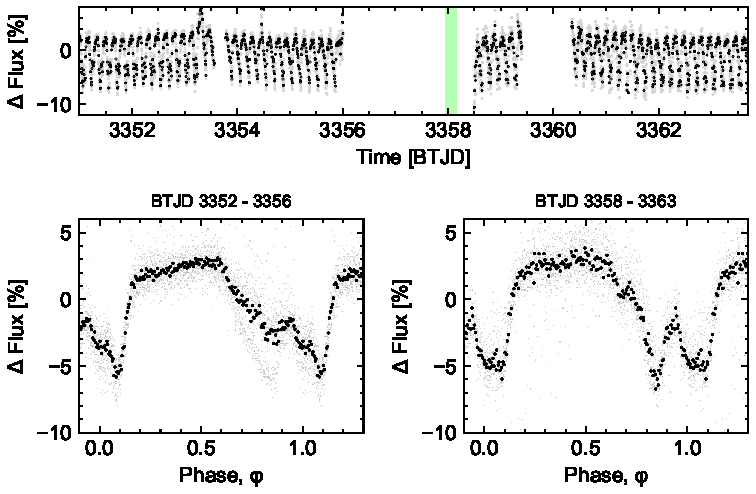
\includegraphics[width=0.99\textwidth]{figures/sf1.pdf}
  \caption{Photometric evolution of TIC 141146667 near the Keck/HIRES
  observation (green bar). 
  {\bf a,} TESS simple aperture photometry.  The main data gaps were
  caused by scattered light from the Earth (BTJD 3356-3358.5) and Moon
  (BTJD 3359.5-3360.5).  Raw two minute data are in gray; black
  time-averages to ten minute sampling.
  {\bf b-c,} Folded light curve before and after spectroscopy.  Raw
  two minute data are in gray; black phase-averages to 100 points per
  cycle.  During BTJD 3352-3356, a state switch occurred near BTJD
  3353, in which the dip at $\phi$$\approx$0.8 disappeared.  While the
  large eclipse feature was present both before and after the HIRES
  sequence, its photometric shape evolved during the data gap.
  }
  \label{fig:fulllc}
\end{figure}

{\it Photometry:} TESS observed TIC~141146667 ($T$=13.3) in Sectors 14,
15, 21, 41, 48, and 75.  Two-minute data were acquired during Sectors
41, 48 (TESS DDT039, PI: Kunimoto), and 75 (TESS Program G06030, PI:
Bouma).  The data from Sectors 14, 15, and 21 had 30-minute cadence,
which smears sharp features over the $<$4\,hour period (see
\cite{Gunther2022}).  The field is not crowded:  the nearest known
star, TIC~141146666 ($T$=14.5), is 25$''$ from TIC~141146667 and is
photometrically stable in the pixel-level TESS data.

Extended Data Figure~\ref{fig:fulllc} shows the TESS Sector~75 data acquired near
the epoch of spectroscopy.  The gap in coverage from BTJD
3356.0~-~3358.5 occurred because the Earth was within 25$^\circ$ of
the TESS camera's boresight, yielding high levels of scattered light;
this gap included the Keck/HIRES observation epoch (green bar).  From
BTJD 3359.4~-~3362.0, the Moon then passed within 25$^\circ$ of the
camera's boresight.  Based on the observed level of scattered light in
the optimal TIC~141146667 aperture, we manually masked out times from
3359.40~-~3360.13, and judged the remainder of the data during the
lunar approach to be usable.  Small data gaps from BTJD
3353.55~-~3353.77 and from BTJD 3360.12~-~3360.33 were caused by data
downlinks at the spacecraft's perigee and apogee, respectively.

Extended Data Figure~\ref{fig:fulllc} shows that a large, complex eclipse
feature was present before and after the HIRES data were
acquired.  From BTJD 3352~-~3356, this eclipse had two sharp local
minima;  the local minimum at $\phi$$\approx$0.8 disappeared following
the flare at BTJD 3353, yielding an eclipse more closely resembling a
long ``V'' than a ``W''.  Similar state changes have previously been
noted and discussed \cite{Stauffer2017,Bouma2024}.  The photometric
shape therefore evolved during the twelve cycles spanning the
3356~-~3358 gap, since the average shape from 3358-3363 more
closely resembles the initial ``W''.



{\it Spectroscopy:}
We observed TIC~141146667 ($V$=16.2) with Keck/HIRES for five hours
during the second half of the night, spanning 17 February 2024 10:47
to 16:13 (UT).
The star's airmass over this window spanned $z$=1.2-2.2, and we opted
for a fixed 15 minute cadence over the entire sequence, except for a
final 10 minute exposure due to increasing sky brightness at sunrise.
We observed without the iodine cell and used the C2 decker
(0$\farcs$86$\times$14$\farcs$0) in the red instrument configuration,
yielding a spectral resolution $R$$\approx$45{,}000 ($\delta
v$$\approx$6.7\,\kms; $\delta v / v_{\rm eq}$$\approx$0.05).  We binned
the CCD readout by a factor of three in the spatial dimension, yielding
$\approx$1,000 photons (S/N=33) per pixel in the continuum at 6500\,\AA,
at minimum airmass.  Strong winds contributed to 1\farcs2$\pm$0\farcs2
seeing over the night, but conditions were otherwise favorable.  We
reduced the echelleogram to a one-dimensional spectrum using the
standard techniques of the California Planet Survey \cite{Howard2010}.
Figure~\ref{fig:spec}b shows the result in the vicinity of H$\alpha$
without any additional processing.


\subsection{Stellar Parameters}\phantom{+}
\label{subsec:stparams}

{\it Radial Velocity}---We measured the radial velocities of TIC~141146667
from our HIRES spectra using a pipeline that we developed for
rapidly rotating stars.  Our method is based on template-matching
against synthetic spectra produced by the PHOENIX stellar atmosphere
code \cite{Husser2013}.  We used the PHOENIX models with solar
metallicity and alpha element abundances, and calibrated our pipeline
using the standard stars described by \cite{Chubak2012}.  We used
velocity standards spanning spectral types from G2 to M4 (Barnard's
Star), irrespective of rotation rate.  We used \texttt{barycorrpy}
\cite{Kanodia2018} to calculate the velocity corrections due to Earth's
motion around the solar system barycenter and due to Earth's daily
rotation about its axis.  Our analysis code reproduces the systemic
velocities of known velocity standards \cite{Chubak2012} with an RMS of
0.66\,\kms.

For TIC~141146667, we measured the radial velocities using regions near
the K~I (7700\,\AA) resonance line and three TiO bandheads (5160\,\AA,
5450\,\AA, and 5600\,\AA).  We selected these regions because they
provided the best matches between the synthetic and observed spectra.
We then averaged the resulting redshift measurements over each order to
produce the final measurement.  We used the scatter of resulting
velocity measurements between orders to assign the RV uncertainty at
each epoch.  The uncertainty-weighted mean systemic velocity over all
epochs on 17~February~2024 was $\gamma$=0.6$\pm$1.5\,\kms.  The
relative radial velocities about this mean are given in
Table~\ref{tab:rv}.

{\it Viewing Orientation}---We fitted the rotational broadening of the
K~I (7700\,\AA) resonance line using the kernel suggested by
\cite{Gray2008}; taking the mean and standard deviation of the resulting
value over all epochs yielded $v_{\rm eq} \sin i$=138$\pm$8\,\kms,
consistent with the visual line broadening $\Delta
\lambda$$\approx$3\,\AA.  The star's equatorial velocity $v_{\rm eq}$
based on its apparent size and rotation period is 130$\pm$4\,\kms.
While this suggests that the viewing orientation could be nearly
edge-on, the formal constraint is rather weak, with $i$$>$63$^\circ$ at
2$\sigma$ (2.5$^{\rm th}$ percentile of the inclination posterior).

% from calc_max_amplitude_sinusoid_rv_timeseries.py
% from K_to_msini.py, assuming Mstar = 0.18

{\it No Evidence For Binarity}---Any periodicity in the
radial velocity time-series is ruled out at the rotation period for
semi-amplitudes above 2.85\,\kms\ (at 3$\sigma$ confidence).  This
sets an upper limit on the mass of any putative companion at the four
hour period of $m \sin i $$<$2.4\,$M_{\rm Jup}$.  Regarding possible
companions at wider separations, the Gaia DR3 renormalized unit weight
error (RUWE), a proxy for the goodness of fit for a single-source
astrometric model to the Gaia astrometry, is 1.23, within the usual
range for apparently single sources.  There are no resolved companions in
the Gaia DR3 point source catalog.  Finally, we checked the TESS light
curve for evidence of secondary photometric periods by subtracting the
mean CPV signal over each sector and performing a phase-dispersion
minimization analysis \cite{Stellingwerf1978,2021zndo...1011188B}.
There were no secondary periods in the TESS data.  Previous work
\cite{Bouma2024} has shown that about 30\% of CPVs show evidence for
excess noise above the Gaia single-source astrometric model, and about
40\% of CPVs show evidence for unresolved binary companions based on
the presence of secondary photometric periods.  This agrees with
analyses showing that multi-periodic low-mass stars are generally
unresolved binaries \cite{Tokovinin2018}.  Overall, the CPV binary
fraction seems consistent with that for field M dwarfs
\cite{Winters2019}, pointing to a weak or non-existent connection
between the CPV phenomenon and (wide) binarity.  For TIC~141146667
specifically, although we find no evidence for stellar multiplicity, our
data are minimally constraining for the scenario of a low-luminosity
companion ($F_1$/$F_2$$\lesssim$0.1) with apparent separation
below 0$\farcs$1.


\begin{figure}[!t]
  \centering
  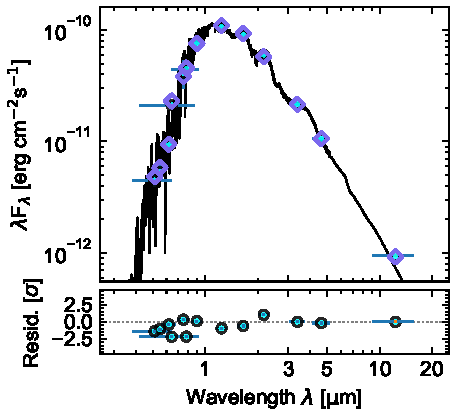
\includegraphics[width=0.7\textwidth]{figures/sf4.pdf}
  \caption{
    Spectral energy distribution of broadband photometric magnitudes
    (filled markers) plotted over the best-fit BT-Settl stellar
    atmosphere model \cite{Allard2012} and the associated photometric
    predictions (empty markers).  This plot was made from an
    adaptation of \texttt{astroARIADNE} \cite{Vines2022}.  The
    photometry extends from the Gaia DR3 blue passband to WISE W3;
    the W4 passband (22 $\mu$m) did not yield a confident detection.
    This fit yields the star's temperature and size.  The lack of
    excess infrared flux relative to the photospheric model sets an
    upper limit on emission from circumstellar dust.
    }
  \label{fig:sed}
\end{figure}

{\it Effective temperature, radius, mass, and spectral
classification}---We adopted the star's effective temperature and
radius measured using the spectral energy distribution (SED) fitting
procedure described by \cite{Bouma2024}.  To summarize, this approach
used \texttt{astroARIADNE} \cite{Vines2022} with the BT-Settl stellar
atmosphere models \cite{Allard2012}, assuming the \cite{Asplund2009}
solar abundances and the \cite{Barber2006} water line lists.  This
approach fitted for the stellar effective temperature, radius,
reddening, surface gravity, metallicity, and distance by comparing the
measured broadband magnitudes against pre-computed model grids.
Specifically, we performed the fit using the broadband magnitudes from
Gaia DR2, APASS, 2MASS, SDSS, and WISE $W1$ and $W2$.  The resulting
best-fit SED is shown in Extended Data Figure Figure~\ref{fig:sed}.  This method has the
most constraining power for the star's effective temperature (2972
$\pm$ 40\,K) and radius (0.42 $\pm$ 0.02\,$R_\odot$); the surface
gravity, metallicity, and reddening are only weakly constrained.  We
determined the star's spectral type to be M5.5Ve by visually comparing
the HIRES spectra against the photometric standards tabulated by
\cite{Bochanski2007}.   This result agrees with the effective
temperature found from the SED fitting \cite{Pecaut2013}.  We measured
the equivalent width of the H$\alpha$ line by fitting a range of
models to the time-averaged line profile shown in
Figure~\ref{fig:spec}, selecting the model that minimized the Bayesian
information criterion, and numerically integrating this best fit model.  
We found a sum of two Gaussians to be the preferred model; our quoted
result, EW$_{{\rm H}\alpha}$=7.2$\pm$0.2\,\AA, comes from numerically
integrating within $|\Delta v/v_{\rm eq}|<1$.  Integrating over the
entire line profile, including the broad wings, would yield EW$_{{\rm
H}\alpha}$=10.2$\pm$0.3\,\AA. Either value would classify the star as
a weak-lined T Tauri \cite{Briceno2019}.

Given the effective temperature, stellar radius, and age range
(35-150\,Myr) derived below, we then estimated the stellar mass by
interpolating against the PARSEC v1.2S isochrones \cite{Chen2014}.
Specifically, we used the distance metric defined in Equation~8 of
\cite{Bouma2024} to select the model mass closest to a given observed
temperature, radius, and age.  This exercise yielded a mass of
$M_\star$=$0.20\pm0.01$\,$M_\odot$ assuming an age of 35\,Myr, or a
mass of $0.25\pm0.01$\,$M_\odot$ assuming an age of 150\,Myr.  These
masses imply Keplerian corotation radii $R_{\rm
cr}/R_\star$=1.75$\pm$0.07 and $R_{\rm cr}/R_\star$=1.89$\pm$0.07,
respectively; this size scale is relevant because it is theoretically
expected to set the inner boundary at which corotating material might
accumulate (e.g.~\cite{Townsend2005,Daley-Yates2024}).  Our final
quoted $M_\star$ and $R_{\rm cr}$ values adopt the average of these
extremes and a quadrature sum of their statistical uncertainties; we
caution however that a more precise age would be needed to resolve the
systematic uncertainties in these parameters.


{\it Age: No Obvious Association Membership}---Previous work
\cite{Bouma2024} has found that over 90\% of CPVs are associated with
known young moving groups based on their positions and kinematics.
TIC~141146667 is in the minority.  We calculated the probability of
TIC~141146667 being part of any nearby known group using
BANYAN\,$\Sigma$ v1.2 \cite{Gagne2018}.  That particular model
classifies it as a field star at $>$99.9\% confidence.  We also
searched the local vicinity of TIC~141146667 for neighbors with
similar projected on-sky velocities using \texttt{comove}
\cite{Tofflemire2021}.  This yielded no strong candidates for
co-moving stars with projected tangential velocities $\Delta v_{\rm
T}$$<$5\,\kms\ that share its isochronal youth.

\begin{figure}[!t]
  \centering
  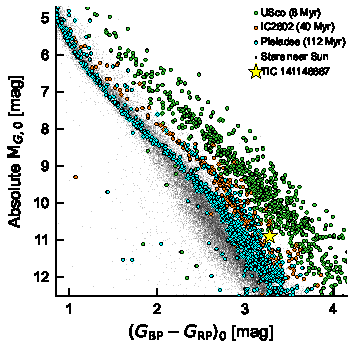
\includegraphics[width=0.7\textwidth]{figures/sf3.pdf}
  \caption{Dereddened Gaia DR3 color vs.~absolute magnitude diagram of
  TIC~141146667 and comparison samples. 
  TIC~141146667 is on the pre-main sequence; stars with the same color
  on the main sequence are $\approx$1.5\,magnitudes
  fainter.  The star's location in this diagram suggests an
  age of 30-150\,Myr.  }
  \label{fig:camd}
\end{figure}


{\it Age: Isochrones}---The color and absolute magnitude of
TIC~141146667 suggest that it is a pre-main sequence M dwarf, similar to
all other known CPVs \cite{Stauffer2017,Stauffer2021,Bouma2024}.  The
star's proximity ($d$=58\,pc) and high galactic latitude
($b$=$+$53$^\circ$) yield negligible interstellar reddening along the
line of sight \cite{Green2019}.  Extended Data Figure~\ref{fig:camd} shows the
location of TIC~141146667 in the color--absolute magnitude diagram
(CAMD) relative to young stellar populations including Upper Scorpius
(USco), IC~2602, and the Pleiades.  To make this diagram, we adopted
the USco members in the $\delta$~Sco and $\sigma$~Sco sub-associations
from \cite{Ratzenbock2023}, and the IC~2602 and Pleiades members from
\cite{Hunt2024}.  We assumed an average $V$-band extinction $A_{\rm
V}$=$\{0.12, 0.11, 0.10\}\,{\rm mag}$ for USco \cite{Pecaut2016},
IC~2602 \cite{Hunt2024}, and the Pleiades \cite{Hunt2024}
respectively, and ages of 8\,Myr \cite{Ratzenbock2023}, 40\,Myr
\cite{Randich2018}, and 112\,Myr \cite{Dahm2015} for each respective
cluster.  We dereddened the photometry using the extinction
coefficients $k_X\equiv A_X/A_0$ tabulated in
\cite{GaiaCollaboration2018}, assuming that $A_0 = 3.1 E(B-V)$.

Extended Data Figure~\ref{fig:camd} shows that TIC~141146667 falls between the USco
and Pleiades sequences, and approximately overlaps IC~2602.  However,
the precision of the implied age is set by the intrinsic scatter of
these calibration sequences; the most luminous stars in the Pleiades of
the same color have a similar absolute magnitude as TIC~141146667.
Previous work \cite{Stauffer2021} has also noted that in the Gaia
passbands, CPVs tend to be photometrically redder and more luminous than
single stars in any given cluster, similar to other rapid rotators.
While this effect complicates any attempt at age inference based on the
Gaia photometry, it suggests that the Pleiades may be a better
comparison population than IC~2602.  We take the star's
location in the color--absolute magnitude diagram to suggest age bounds
$t_{\rm CAMD}$$\sim$30-150\,Myr.


{\it Age: Lithium}---The depletion of lithium due to $^7$Li(p,
$\alpha$)$^4$He burning in the cores of low-mass stars has been studied
for over sixty years \cite{Hayashi1963,Bildsten1997,Burke2004}.
\cite{Wood2023} provided a recent overview: an abbreviated
summary is that sufficiently cool and young M dwarfs show the 6707.8\,\AA\
doublet in absorption, $\gtrsim$10\% below their continua.  However unlike
for Sun-like stars, the continuum for M dwarfs is challenging to define due to
their molecular absorption.  We therefore attempted a lithium measurement by
constructing a wavelength-binned and Doppler-corrected TIC~141146667
spectrum, assigning its uncertainties based on the measured scatter
across the five hour dataset.  We then compared this average spectrum
against the nearest matching M6 template from \cite{Bochanski2007}.  The
data show a small depression near the expected lithium wavelength,
potentially consistent with the $\Delta \lambda$$\approx$3\,\AA\ line
broadening.  This feature nominally yields ${\rm EW}_{\rm
Li}$=71$^{+18}_{-13}$\,m\AA, where the statistical uncertainties are
evaluated using a bootstrap resampling technique from the statistical
uncertainties in the HIRES spectrum.  However, the systematic uncertainties associated
with the continuum normalization are likely comparable to
the amplitude of this feature; we therefore treat the result of this
measurement as a $2\sigma$ upper limit: ${\rm EW}_{\rm Li}$$<$107\,m\AA.


\begin{figure}[!t]
  \centering
  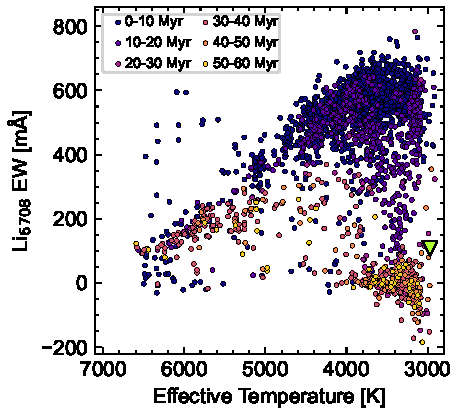
\includegraphics[width=0.7\textwidth]{figures/sf2.pdf}
  \caption{An upper limit on photospheric lithium for TIC~141146667
  (green triangle) yields a lower bound on the star's age of
  $\gtrsim$20\,Myr.  Comparison stars are from the Gaia-ESO survey
  \cite{Jeffries2023}; rich clusters in each age bin include NGC\,2264
  (4.5\,Myr), $\lambda$~Ori (8.7\,Myr), ${\rm \gamma}^2$\,Vel
  (16.4\,Myr), NGC\,2547 (35.0\,Myr), IC\,2602 and IC\,2391 (42.0\,Myr),
  and NGC\,2451A (50.0\,Myr). }
  \label{fig:liew_population}
\end{figure}



Despite uncertainties in the details, what can be stated with confidence
is that lithium is not abundant in the spectrum of TIC~141146667.
Extended Data Figure~\ref{fig:liew_population} compares our upper limit against the
equivalent width measurements reported by \cite{Jeffries2023}
based on the Gaia-ESO spectroscopic survey; Extended Data Figure~\ref{fig:hirescuts}
shows the associated raw spectra.  If the star were $\lesssim$20\,Myr
old, at its temperature we would expect to see lithium in abundance
($>$400\,m\AA).  Since we do not, we can set an empirical bound on the
lithium-derived age of $t_{\rm Li,emp}$$\gtrsim$20\,Myr.  The
\cite{Feiden2016} lithium isochrones provide a point for theoretical
comparison, and suggest that since $M_{\rm K}$$\approx$6.67\,mag,
$t_{\rm Li,th}$$\gtrsim$35\,Myr is the theoretical age at which
complete depletion occurs in a star with this luminosity (see
e.g.~Figure 7 from \cite{Wood2023}).




{\it Age: Summary}---The main indicators for the youth of
TIC~141146667 are {\it i)} that it is a complex periodic variable, and
{\it ii)} that it is 1.5 magnitudes brighter (four times more
luminous) than main sequence stars of the same color, while showing no
indicators for binarity.  Being a CPV suggests that the star is young
because a previous CPV search unbiased in age found 90\% of its
detections to be in $\lesssim$200\,Myr old clusters \cite{Bouma2024};
the remaining 10\% were not associated with any coeval
population.
Similarly, studies of rotation in $\lesssim$100\,Myr clusters serendipitously found
$\approx$50-100 examples of the class
\cite{Rebull2016,Stauffer2017,Stauffer2018,Rebull2018,Zhan2019,Rebull2020,Stauffer2021,Rebull2022,Popinchalk2023},
whereas analogous studies of Praesepe and the Hyades did not report
any evidence for CPVs in a set of approximately one thousand
$\approx$700\,Myr stars \cite{Rebull2017,Douglas2019,Rampalli2021}.
Regarding the isochronal age constraint, the Pleiades (112\,Myr,
\cite{Dahm2015}) shows a few stars of equal luminosity and the same
temperature, suggesting a photometric isochronal age upper limit
$\lesssim$150\,Myr.  The weak lithium absorption suggests an age of at
least 20\,Myr based on an empirical comparison using Gaia-ESO spectra,
or at least 35\,Myr based on the \cite{Feiden2016} isochrones.  These
considerations yield our adopted age range of 35-150\,Myr.




\subsection{Spectroscopic Variability}\phantom{+}
\label{subsec:specvar}

\begin{figure}[!t]
  \centering
  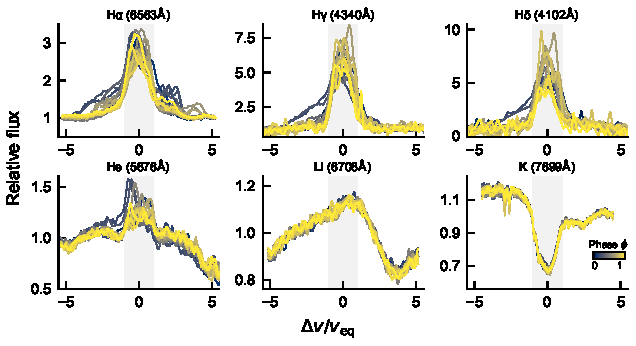
\includegraphics[width=\textwidth]{figures/sf5.pdf}
  \caption{Time evolution of select regions in the Keck/HIRES
  spectra from 17 February 2024.
  We made this plot by applying a windowed outlier rejection to remove
  cosmic rays and then smoothing each spectrum with a Gaussian filter.
  The horizontal axis shows the velocity relative to each
  line's rest wavelength, normalized by the stellar equatorial
  velocity.  
  H$\alpha$ is the only Balmer line to show periodic variability of
  the form seen in Figure~\ref{fig:spec}.
  The He 5876\,\AA\ line shows a time-dynamic blueshift that 
  differs from the Balmer lines.
  Li 6708\,\AA\ shows no obvious absorption.
  }
  \label{fig:hirescuts}
\end{figure}

Extended Data Figure~\ref{fig:hirescuts} shows a few regions of interest in the
HIRES spectra, which cover 3650-7960\,\AA.  Higher order Balmer lines
including H$\gamma$ and H$\delta$ ($n=5\rightarrow2$ and
$n=6\rightarrow2$) do show variability outside the line core.
However, this variability is not clearly periodic in the same manner
as the emission seen in H$\alpha$.  This could be because there are
insufficient hydrogen ions in the relevant excited states, or because
the spectra have lower precision in these bluer regions.  The Ca HK
doublet is also detected in emission, while the continuum near it is
not.  Chromospheric emission from the magnesium triplet is also
detected, but these lines are too blended to be usable.

Extended Data Figure~\ref{fig:hirescuts} provides a novel view on the
blue excess that appeared at $\phi$$\approx$0.2 in H$\alpha$, H$\gamma$,
H$\delta$, and He 5876\,\AA.  At the same epoch, H$\alpha$ additionally
shows a red clump of emission, and H$\gamma$ and H$\delta$ are also
broadened on the red wing.  The rise of this emission in $<$15\,minutes
might suggest a more sudden flow, rather than a stable, periodic
component.  For instance, a stellar flare might be connected to such a
sudden rise.  However, this idea seems incompatible with the sinusoidal
emission seen later from $\phi$$\approx$0.5-1.0, and with the fact that
flares typically excite iron lines in the blue HIRES orders, which are
not observed.  More time-series spectroscopy would be needed to clarify
this type of variability, in particular whether it is periodic or
stochastic.

Finally, the Li\,\textsc{I} 6708\,\AA\ doublet, which shows no obvious
absorption, as well as the broad K\,\textsc{I} 7699\,\AA\ resonance
line are both visible in Extended Data Figure~\ref{fig:hirescuts}.  In the latter,
narrow telluric absorption features overlap the blue wing of the line.
Neither of these regions shows any notable variability.



\subsection{Detailed Behavior of H$\alpha$: Model and Implications}\phantom{+}
\label{subsec:halpha}

\begin{figure}[!tp]
  \centering
  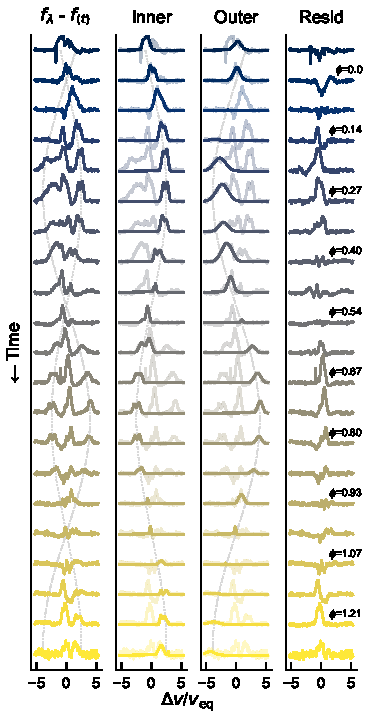
\includegraphics[width=0.55\textwidth]{figures/sf6.pdf}
  \caption{Time-variable fit to H$\alpha$ line profiles.
  {\it Left column:} Raw spectrum at each epoch $f_{\lambda}$ minus
  the time-averaged spectrum $f_{\langle t \rangle}$ (as in
  Figure~\ref{fig:spec}e).
  Underplotted sinusoids are not fits; they are meant to guide the eye.
  {\it Middle columns:} Model of emission from the inner clump (sum of
  two gaussians) and the outer clump (single gaussian), plotted over
  the data.
  {\it Right column:} Residual of the left column after subtracting
  the sum of the two middle columns, leaving variability in the line
  core.  
  \S~\ref{subsec:halpha} discusses the use of this model.
  }
  \label{fig:halphamodel}
\end{figure}

{\it A model for the time-dynamic H$\alpha$ spectrum}---While
Figure~\ref{fig:spec} shows that clumps of circumstellar material
exist around TIC~141146667, there is value in quantifying the exact
orbital periods, velocities, and velocity dispersions of these clumps.
These quantities can constrain the physical dimensions of the emitting
region, and can also clarify whether the spectroscopic period agrees
with the photometric period.

Given that a full radiative transfer simulation was outside our scope,
we opted to construct a phenomenological model aimed at capturing 
the emission from the circumstellar material.  We did this by
fitting each spectral epoch with a multi-component
gaussian, after having subtracted the time-average line profile as in
Figure~\ref{fig:spec}e.  The results of this exercise are shown in
Figure~\ref{fig:halphamodel}; details in the implementation and
interpretation follow.

To implement the model, we assumed that the ``inner'' ($K_{\rm
inner}$$\approx$2.5\,$v_{\rm eq}$) clump would be well-fit by a sum of
two gaussians because it is visually double-peaked in the raw
data from $\phi$=0.15-0.35 and $\phi$=0.65-0.85
(Figure~\ref{fig:spec}b).  We assumed that the ``outer'' ($K_{\rm
outer}$$\approx$3.9\,$v_{\rm eq}$) clump would be better fit by a
single gaussian, based on its behavior from $\phi$=0.6-0.9.  Each
gaussian component has three free parameters at each spectral epoch:
the mean $\mu$, standard deviation $\sigma$, and amplitude $A$.
We labelled the inner component's two gaussians $i=\{ 0, 1 \}$,
and the single outer component as $i=2$.  Given the complexity of the
line profile data (Figure~\ref{fig:halphamodel} left column), the
likelihood function for this model is multimodal.  We therefore
imposed the prior constraints that $A_i \sim \mathcal{U}[0,1]$,
$\sigma_i/v_{\rm eq} \sim \mathcal{U}[0,1]$, and further assumed
$\mu_i(t) \sim
\mathcal{U}[
  K_{\rm inner}\sin(\phi(t)) - v_{\rm eq},
  K_{\rm inner}\sin(\phi(t)) + v_{\rm eq}
]$
for the inner two components, and
$\mu_2(t) \sim
\mathcal{U}[
  K_{\rm outer}\sin(\phi(t) + \pi) - 2v_{\rm eq},
  K_{\rm outer}\sin(\phi(t) + \pi) + 2v_{\rm eq}
]$
for the outer component.  This prior on the means mitigates 
multimodality in the likelihood by requiring the mean velocity of each
component to be within a one or two $v_{\rm eq}$ of the time-variable
sinusoid suggested by visual inspection.  We fitted each component to
the data {\it independently} using scipy's non-linear least squares
\texttt{curve\_fit} implementation \cite{Virtanen2020}, and scaled the
resulting parameter covariance matrix by a constant factor to match
the sample variance of the residuals.  The resulting means,
amplitudes, and standard deviations for each component are given in
Extended Data Table~\ref{tab:halphamodelparams}.

Caution is required in interpreting this model's results.  
At certain epochs the most significant spectral
feature around any component's prior is not statistically significant.
During such epochs, e.g.~the ``outer'' clump at $\phi$=1.07,
the model fits noise, not signal.  At other times, the model
underfits.  For instance, the sudden blue rise near $\phi$=0.2 is 
poorly described by a gaussian; the assumed functional form is one of
convenience.  Finally, the model fits the $i=\{ 0, 1 \}$, and $i=2$
components independently.  At $\phi$=0.0 and 1.0,
Figure~\ref{fig:halphamodel} suggests that the emission
might come from either the inner or outer components.
Physically however, at this epoch the inner clump
is in transit, and the outer clump is passing behind
the star.  At $\phi$=0.0, the double-peaked
emission profile also matches that seen shortly afterward (at
$\phi$=0.14) when the
inner clump is viewed off-disk.  A physical interpretation of the
model would therefore discard the outer clump results at this
particular epoch, because its emission would be blocked by the star.

\begin{figure}[!t]
  \centering
  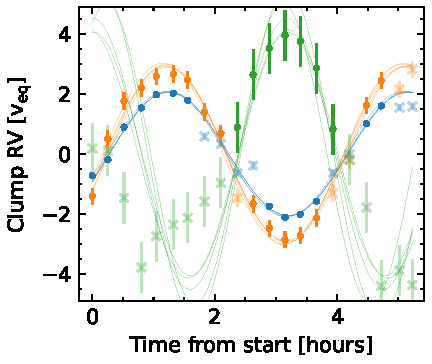
\includegraphics[width=0.7\textwidth]{figures/sf7.pdf}
  \caption{Orbits fit to mean radial velocities (RVs) extracted from 
  H$\alpha$ profile fits in Figure~\ref{fig:halphamodel}.
  Radial velocities on the vertical axis are in units of the
  equatorial velocity, $v_{\rm eq}$=130\,\kms.
  Each marker denotes the best-fit mean at a given epoch.
  Solid circles were adopted in the fits; transparent X markers
  were excluded due to concerns about their reliability
  (see text).  The inner double-peaked clump is shown in
  black and orange; the outer clump is shown in green.  Five draws from
  each posterior probability distribution are shown.}
  \label{fig:orbits}
\end{figure}

Accounting for these caveats, we used the results from Extended Data
Table~\ref{tab:halphamodelparams} to quantify the orbital periods and
velocity semi-amplitudes of the clumps.
Figure~\ref{fig:orbits} shows the results assuming circular
orbits; considering the Bayesian information criterion, we found no
reason to prefer eccentric orbits.  By visually
inspecting Extended Data Figure~\ref{fig:halphamodel}, we excluded
epochs where our gaussian profile fitting failed to either detect or
else adequately represent the circumstellar emission.  We then used
NumPyro to sample the Gaussian likelihood for a Keplerian orbit
with the NUTS algorithm \cite{Phan2019}.  We used the measurement
uncertainties from each estimated mean radial velocity value and
included an additional jitter term in quadrature.  This procedure
yielded orbital periods and semi-amplitudes of
$P_0$=$3.92\pm0.03$\,hr, $K_0/v_{\rm eq}$=2.07$\pm$0.04;
$P_1$=$3.92\pm0.06$\,hr, $K_1/v_{\rm eq}$=2.88$\pm$0.10;
and $P_2$=$3.88\pm0.20$\,hr, $K_1/v_{\rm eq}$=3.88$\pm$0.25.
The periods for the inner double-peaked clump are therefore consistent with the
photometric $3.930\pm0.001$\,hr period within a precision of two
minutes.  The ``period'' for the outer clump is ambiguous because the
H$\alpha$ data only support the idea of a periodic orbit of material
well-fit by gaussian emission from $\phi$$\approx$0.5-1.0.  From
$\phi$=0-0.2, there is no detectable emission, and from
$\phi$=0.2-0.4, the emission spans 1-4\,$v_{\rm eq}$ without taking a
clear gaussian shape.  While the outer-most edge of this
$\phi$=0.2-0.4 emission provides a plausible match to the expectation
of a circular orbit, the idea of invoking a particular functional form
for this component seems fine-tuned.  We instead emphasize that
although this emission is present, its variability in time is 
inconsistent with the idea of a stable clump of material.
Additional observations would be needed to conclusively
determine whether or not this component of the system is long-lived.


{\it Physical dimensions of the emitting region}---The measured velocity
widths from the circumstellar emission contain information about the
size of the emitting region via the condition for rigid corotation.
Consider a clump in cylindrical coordinates with arbitrary radial extent
$r$, azimuthal extent $\ell$, and height $z$.  A range of shapes,
including an ``arc'' with $\ell \gg r$, a ``spoke'' with $r \gg \ell$, and
a ``blob'' with $r \approx \ell \approx z$ are all a priori possible.
However, at quadrature, the observed velocity width of emission is
sensitive to the radial extent of the circumstellar material.  At
mid-transit, the observed velocity width is sensitive to the azimuthal
extent.  An arc configuration would minimize the observed velocity width
$\sigma$ at quadrature, and maximize it during transit, with
$\gtrsim$100\,\kms\ variations in between.  This is not observed.   The
arc geometry, and by a similar argument the spoke geometry, can thus be
discarded.  

At quadrature, the inner clumps show $\sigma_i$$\approx$0.24\,$v_{\rm
eq}$, implying that 68\% of the emission comes from a volume with length
in the radial dimension $r_i$=$2\sigma_i / \Omega$$=$0.48\,$R_\star$,
and that 95\% of the emission comes from within 0.96\,$R_\star$.  These
values have relative uncertainties of $\approx$5\%, based on the
uncertainties in the measured velocity dispersions.  The two inner
clumps are centered at orbital distances of 2.07\,$R_\star$ and 2.88\,$R_\star$.
There is therefore physical overlap in their spatial distributions.
These two clumps could in fact be a single clump with an optically thick
H$\alpha$ line core.  Regardless of this nuance, the implication is that
the full length in the radial dimension of these two inner emitting
clumps is approximately equal to the star's diameter.  At mid-transit, these
inner clumps likely have a similar velocity dispersion, although with
greater uncertainty due to the differences between the $\phi$=0 and
$\phi$=1 transits (see Extended Data Figure~\ref{fig:halphamodel}).
This suggests a 1$\sigma$ emission contour in the azimuthal dimension
with a length of $\ell$$\approx$0.5\,$R_\star$.

The vertical height of the emitting region is less constrained because
the system is consistent with being viewed edge-on.  However, one
constraint does come if one assumes that the TESS transit depth scales
with the projected H$\alpha$ emission area $\ell z$.  
More specifically,
one can evaluate an ``effective area'' blocked by a two-dimensional
gaussian blob passing over a star by integrating the local gaussian
weight over the stellar surface.  For instance, if
$\ell$$\approx$$z$$\approx$0.24\,$R_\star$, then
$\iint \exp \left(
  -\left( x^2/2\sigma_x^2 + y^2/2\sigma_y^2 \right)
\right) {\rm d}x \, {\rm d}y$
suggests 11.5\% of the star being ``blocked'', a geometric factor which
would need to be in turn multiplied by an unknown opacity factor to
produce the observed transit depth ($\delta$$\approx$5\%).  In general
though, there is a degeneracy between $z$ and this opacity factor; larger
vertical heights are allowed for lower optical depths in absorption, and
vice-versa.  
This constraint also implicitly assumes that the optically thick
material is well-mixed with the hydrogen, which may not be accurate.


\subsection{Properties of the Plasma and Magnetospheric Environment}\phantom{+}
\label{subsec:gas}

The physical conditions inside the plasma clumps, in particular the
hydrogen number density, plasma temperature, ionization fraction, and
magnetic field strength can be estimated from the available data.
We caution that the following estimates are order of magnitude
calculations that assume a simple uniform-density plasma: detailed
considerations of radiative transfer are a worthy topic for future
work, but are beyond the scope of this article.

Circumstellar H$\alpha$ emission might be sourced either from resonant
scattering of stellar H$\alpha$ photons, or from radiative
recombination.  We neglect scattering because Figure~\ref{fig:spec}
and Extended Data Figure~\ref{fig:hirescuts} show the amplitude of the circumstellar
H$\alpha$ emission varying by a factor of $\approx$5, in a manner
uncorrelated with any variability in the chromospheric line core.  The
volume emissivity under case B recombination can be written
\begin{equation} j_{\rm H\alpha} = n_{\rm e} n_{\rm p} \alpha^{\rm
eff}_{\rm H\alpha} h \nu_{\rm H\alpha}, \end{equation} where $n_{\rm
e}$ and $n_{\rm p}$ are the electron and proton densities, and
$\alpha^{\rm eff}_{\rm H\alpha}$ is the effective recombination
coefficient, defined to include all recombination routes that produce
an H$\alpha$ photon.  For hydrogen with temperatures between
1,000-10,000\,K, $\alpha^{\rm eff}_{\rm H\alpha}$ is typically on the
order of $10^{-12}$ to $10^{-13}$\,cm$^3$\,s$^{-1}$
\cite{Hummer1987,Draine2011}.  Neglecting the effects of atoms other
than hydrogen, we can assume an ionization fraction $x$, such that
$n_{\rm e} = n_{\rm p} = x n_{\rm H}$, for $n_{\rm H}$ the hydrogen
number density.  Let $L_{\rm H\alpha} = j_{\rm H\alpha} V$, for $V$
the volume of the emitting hydrogen.  The luminosity of circumstellar
hydrogen emission, $L_{\rm H\alpha}$, is an observable: our SED
fitting routine yields $L_\star$$\approx$0.012\,$L_\odot$, which
implies that the stellar H$\alpha$ line radiates at
$\approx$1.0$\times$$10^{28}$erg\,s$^{-1}$.  The luminosity of the
clumps $L_{\rm H\alpha}$ are of order one tenth that of the star.  If
we approximate the emitting volume as a homogeneous sphere of radius
$r$, we can write
\begin{align}
  n_{\rm H} &= 
  1 \cdot 10^{11}\,{\rm cm}^{-3}
  \left(
    \frac{0.5}{x}
  \right)
  \left( 
    \frac{ L_{\rm H\alpha} }{ 10^{27}\,{\rm erg\,s^{-1}} }
    \frac{ 10^{-13}\,{\rm cm^{3}\,s^{-1}} }{ \alpha^{\rm eff}_{\rm H\alpha} }
  \right)^{1/2}
  \left(
    \frac{ 0.1\,R_\odot }{ r }
  \right)^{3/2}.
  \label{eq:numdensity}
\end{align}
For a uniform density clump, this suggests a total gas mass of $M_{\rm
gas}\approx 8\times10^{16}$\,g.
We emphasize that Equation~\ref{eq:numdensity} in intended to provide
only an order of magnitude estimate for the number density implied by
the observed H$\alpha$ emission.  In detail, the effective
recombination rate and the ionization fraction each vary with density
and temperature; a more thorough estimate would iteratively solve the
equations of detailed balance and radiative transfer
(e.g.~\cite{CollierCameron1989} Figure~8), and potentially also
consider departures from local thermodynamic equilibrium.

Finally, a constraint on the magnetic field strength at the site of
the clump follows from the requirement that the magnetic pressure
exceed the thermal pressure, $B_{\rm c}^2 / 8\pi > n_{\rm H} k T$.  Although
we do not know the plasma temperature, if it were significantly beyond
1,000-10,000\,K, we would either fully ionize the hydrogen, or not
ionize enough of it.  The field strength at the clump must therefore
exceed
\begin{equation}
  B_{\rm c} \gtrsim 1\,{\rm G}
  \left(
  \frac{n_{\rm H}}{1\times10^{11}\,{\rm cm}^{-3}}
  \frac{T}{3000\,{\rm K}}
  \right)^{1/2}.
\end{equation}
Given that the average surface magnetic field strengths of low-mass
stars have been measured to span hundreds to thousands of Gauss
\cite{Donati2009,Kochukhov2021,Reiners2022}, this bound is easily met at
orbital distances of 2-4\,$R_\star$.

\subsection{Upper and Lower Bounds on Dust}\phantom{+}
\label{subsec:dust}

The material's composition -- either pure plasma, or a dusty plasma --
is not known.  The idea of dust being present seems plausible given
observations of chromatic transits in analogous objects
\cite{Tanimoto2020,Gunther2022,Koen2023}.  However, this scenario is
highly constrained.  An upper limit on the amount of hot dust follows
from the lack of an infrared excess.  A lower limit follows if one
assumes that most of the broadband optical depth comes from dust
absorption and scattering, rather than any radiative processes
associated with the plasma.

Regarding the upper limit, Extended Data Figure~\ref{fig:sed} shows the SED.  While
AllWISE \cite{Cutri2014} yielded a confident W3 detection
(9.8$\sigma$) consistent with the photospheric extrapolation from bluer
bandpasses, the W4 extraction yielded only a marginal indication
(1.7$\sigma$) of detectable flux.  Similar to other CPVs
\cite{Stauffer2017,Bouma2024}, the photometric uncertainties from WISE
W1 and W2 allow at most a $\lesssim$2\% excess at 3-5\,$\mu$m relative
to the stellar photosphere, and a $\lesssim$5\% excess at 10\,$\mu$m
(W3).  To estimate the implied mass bound, we assume a dust
temperature $T_{\rm d}$=1500\,K, typical for dust near the star (see
\cite{Zhan2019} for discussion regarding dust sublimation).  We then
treat emission from the dust and star as Planck functions, and require
$L_{\rm d} < f L_\star$, where the factor $f$ is set by the
photometric precision of WISE and $L_{\rm d}$ is the bolometric dust
luminosity.  Given the reported uncertainties, we numerically find
$f<6\cdot$10$^{-3}$.  From the Stefan-Boltzmann law we can then write
$A_{\rm d} < f (T_\star / T_{\rm d})^4 Q_{\rm em}^{-1} (4\pi
R_\star)^2$, for $A_{\rm d}$ the total emitting surface area of the
dust, and $Q_{\rm em}$ an emission efficiency parameter.  Converting
this constraint to a dust mass requires an assumption regarding the
grain properties.  We assume a grain density $\rho_{\rm
d}$=3\,g\,cm$^{-3}$ typical for silicate grains, a fixed grain size
$a$=1\,$\mu$m, and no self-absorption.  This enables the assumption
that $A_{\rm d} = N \pi a^2$, for $N$ the total number of dust grains.
This in turn yields an upper limit on the dust mass of
\begin{equation}
  M_{\rm dust} \lesssim 4 \cdot 10^{17}\, {\rm g}\ 
  \left( \frac{f}{6\cdot10^{-3}} \right)
  \left( \frac{T_\star}{3000\,{\rm K}} \frac{1500\,{\rm K}}{T_{\rm d}} \right)^4
  \left( \frac{Q_{\rm em}}{1} \right)^{-1}
  \left( \frac{R_\star}{0.4\,R_\odot} \right)^2
  \left( \frac{a}{1\,\mathrm{\mu m}} \right)
  \left( \frac{\rho_{\rm d}}{3\,\mathrm{g\,cm^{-3}}} \right).
\end{equation}

The analogous lower limit follows from requiring the optical depth
from absorption and scattering $\tau$ to be at least unity.  The
optical depth can be written $\tau = n \sigma \ell$, where
$\sigma$ is the cross-section, $n$ is the number density, $\ell$ is
the path length.  For spherical dust
grains in the optical, $\sigma = Q_{\rm ext} \pi a^2$, where $Q_{\rm
ext}$ is the extinction efficiency parameter, tabulated e.g.~by
\cite{Croll2014} in their Figure 13.  \cite{Sanderson2023} calculated
the relevant cloud mass for this problem assuming a spherical dust
clump of size $r$, and they found
\begin{equation}
  M_{\rm dust} \gtrsim 2 \cdot 10^{15}\, {\rm g}\ 
  \left( \frac{\tau}{1} \right)
  \left( \frac{Q_{\rm ext}}{3} \right)^{-1}
  \left( \frac{r}{0.1\,R_\star} \frac{R_\star}{0.4\,R_\odot} \right)^2
  \left( \frac{a}{1\,\mathrm{\mu m}} \right)
  \left( \frac{\rho_{\rm d}}{3\,\mathrm{g\,cm^{-3}}} \right).
\end{equation}

Three relevant objects for comparison include solar
prominences, planetesimals, and comets.  Prominences of the Sun have
gas masses of $10^{14}$\,g-$10^{16}$\,g \cite{VialEngvold2015}.
A planetesimal of mass $\approx$10$^{15}$\,g with a bulk density of
1\,g\,cm$^{-3}$ would have a diameter of order one kilometer.
Halley's comet has a mass of order $10^{17}$\,g \cite{Rickman1989}, of
which $\sim$$10^{14}$\,g is shed per orbit, most of which inspirals
toward the Sun due to Poynting-Robertson drag.

To summarize, if dust is responsible for
the broadband variability of CPVs, it would need to be concentrated in
clumps with masses in the range of $10^{15}$-$10^{17}$\,g.  Given
$M_{\rm gas}$$\approx$8$\times$10$^{16}$\,g from
\S~\ref{subsec:gas}, the allowed dust masses imply $M_{\rm
gas}/M_{\rm dust}$ ranges of 1-100.  More careful measurements of this
ratio---in particular by inferring the dust mass through high
precision infrared spectrophotometry---could provide a path for
distinguishing the scenario of a trapped stellar outflow from an
accumulation of externally-sourced material.  While there are several
plausible external sources, feeding through a low-mass disk in
particular cannot be ruled out based on typical disk depletion times
\cite{Haisch2001}.  Observations of infrared excesses and accretion
signatures in low-mass stars tens of millions of years old suggest a
broad lifetime distribution for such disks
\cite{Silverberg2020,Lee2020,Gaidos2022,Pfalzner2024}.


%%%%%%%%%%%%%%%%%%%%%%%%
% Supplementary Tables %
%%%%%%%%%%%%%%%%%%%%%%%%

\begin{table}
    \centering
    \begin{tabular}{lcr}
    \hline 
    \hline
    Parameter & Host & Source \\
    \hline 
    \multicolumn{3}{c}{Identifiers} \\
    \hline
    TIC & 141146667 & TESS \\
    Gaia & 860453786736413568 & Gaia\ DR3 \\
    \hline
    \multicolumn{3}{c}{Astrometry \& Radial Velocity} \\ 
    \hline
    $\alpha_{2000}$ & 11:05:15.09   & Gaia\ DR3 \\
    $\delta_{2000}$ & +59 15 05.57  & Gaia\ DR3 \\
    $\mu_{\alpha}$ (mas yr$^{-1}$ ) & -73.933 $\pm$ 0.022 & Gaia\ DR3 \\
    $\mu_{\delta}$ (mas yr$^{-1}$ ) &  32.262 $\pm$ 0.024 & Gaia\ DR3 \\
    $\pi$ (mas)                     &  17.324 $\pm$ 0.025 & Gaia\ DR3 \\
    RUWE                            &  1.23               & Gaia\ DR3 \\
    RV (\kms)                       & 0.61 $\pm$ 1.47     & HIRES \\
    \hline
    \multicolumn{3}{c}{Photometry} \\
    \hline
    $TESS$ (mag)                    & 13.283 $\pm$ 0.010 & TIC8\     \\
    $G$ (mag)                       & 14.701 $\pm$ 0.002 & Gaia\ DR3 \\
    $G_{\rm BP}$ (mag)              & 16.664 $\pm$ 0.008 & Gaia\ DR3 \\
    $G_{\rm RP}$ (mag)              & 13.398 $\pm$ 0.006 & Gaia\ DR3 \\
    $G_{\rm BP}$-$G_{\rm RP}$ (mag) &  3.276 $\pm$ 0.010 & Gaia\ DR3 \\
    $J$ (mag)                       & 11.401 $\pm$ 0.022 & 2MASS     \\
    $H$ (mag)                       & 10.793 $\pm$ 0.021 & 2MASS     \\
    $K_s$ (mag)                     & 10.473 $\pm$ 0.016 & 2MASS     \\
    $W1$ (mag)                      & 10.276 $\pm$ 0.023 & ALLWISE   \\ % Cutri+2013 II/328/allwise
    $W2$ (mag)                      & 10.070 $\pm$ 0.020 & ALLWISE   \\
    $W3$ (mag)                      &  9.838 $\pm$ 0.045 & ALLWISE   \\
    %$W4$ (mag)                      &  8.392 $\pm$ NOUNC & ALLWISE \\
	  %
    % NOTE: ROSAT is an emitter.  GALEX detection.
    % ROSAT: 3.25e-13 mW/m^2 = erg/cm^2/s
    % Ofek+2011 1.4Ghz emitter.  Helfand+2015 ditto.  Bruzewski+2021.
    \hline
    \multicolumn{3}{c}{Physical Properties} \\
    \hline
    $T_{\rm eff}$ (K) & 2972 $\pm$ 40 & SED fit \cite{Bouma2024} \\
    $R_\star$ ($R_{\odot}$) & 0.42 $\pm$ 0.02 & SED fit \cite{Bouma2024} \\
    $L_\star$ ($L_\odot$) & 0.0126 $\pm$ 0.0012 & SED fit \cite{Bouma2024} \\
    $P_{\rm rot}$ (hours) & 3.930 $\pm$ 0.001 & TESS \\ 
    $v_{\rm eq}$ (\kms)  &  130$\pm$4  & Derived \\
    $v_{\rm eq} \sin i_\star$ (\kms) & 138 $\pm$ 8 & HIRES \\
    $i_\star$($^\circ$) & $>$63 & Derived \\
    $A_V$ (mag) & 0 & \cite{Green2019} \\
    $M_\star$ ($M_{\odot}$)  & 0.22 $\pm$ 0.02  & PARSEC \cite{Chen2014}\\
    ${\rm EW}_{\rm Li}$ (m\AA) & $<$107 & HIRES (2$\sigma$)\\
    $t_{\rm CAMD}$ (Myr) & 30-150 &  Gaia DR3 \\
    $t_{\rm Li,emp}$ (Myr) & $>$20 &  HIRES, \cite{Jeffries2023} \\
    $t_{\rm Li,th}$ (Myr) & $>$35 &  HIRES, \cite{Feiden2016} \\
    $t_{\rm adopted}$ (Myr) & 35-150 &  -- \\
    \hline
    \end{tabular}
		\caption{Properties of TIC~141146667.  References:
    Gaia DR3 \cite{GaiaDR3}, TESS \cite{Ricker2015},
    TIC8 \cite{Stassun2019}, 2MASS \cite{Skrutskie2006}, ALLWISE
    \cite{Cutri2014}.}
    \label{tab:stparams}
\end{table}


\begin{table}
  \centering
  \begin{tabular}{lcr}
  \hline 
  \hline 
  Time [BJD$_{\rm TDB}$] & RV (\kms) & $\sigma_{\rm RV}$ (\kms) \\
  % from tables/tab_TIC141146667_rel_rv.tex and
  % tables/tab_TIC141146667_times_rounded.csv
  \hline 
  2460357.954919 & 2.73 & 5.86 \\
  2460357.965845 & -4.40 & 2.37 \\
  2460357.976770 & -0.19 & 2.64 \\
  2460357.987698 & 3.84 & 2.87 \\
  2460357.998619 & 7.53 & 7.53 \\
  2460358.009538 & -1.98 & 1.44 \\
  2460358.020462 & 1.02 & 1.21 \\
  2460358.031383 & 0.64 & 7.03 \\
  2460358.042306 & -2.91 & 2.71 \\
  2460358.053228 & 8.93 & 6.75 \\
  2460358.064154 & 5.95 & 8.84 \\
  2460358.075075 & -2.25 & 3.06 \\
  2460358.085996 & 1.84 & 1.34 \\
  2460358.096918 & 2.41 & 8.24 \\
  2460358.107839 & -7.04 & 3.94 \\
  2460358.118760 & -2.24 & 3.07 \\
  2460358.129683 & -2.83 & 7.55 \\
  2460358.140606 & -0.59 & 2.26 \\
  2460358.151527 & 1.84 & 2.91 \\
  2460358.162448 & 4.54 & 3.95 \\
  2460358.173368 & 6.21 & 12.14 \\
  \hline
  \end{tabular}
  \caption{TIC~141146667 radial velocities relative to the systemic
  velocity based on the 7699\,\AA\ resonance line and TiO bandheads.}
  \label{tab:rv}
\end{table}


\begin{sidewaystable}
%\begin{table}
  %\small
  \footnotesize
  \centering
  \begin{tabular}{lccccccccc}
  %\hline 
  %\hline 
  %Time [BJD$_{\rm TDB}$] & RV (\kms) & $\sigma_{\rm RV}$ (\kms) \\
  % from
  % results/halpha_to_rv_timerseries/multigauss_parametertable.tex
  \hline
  BTJD & $\mu_0$ & $\mu_1$ & $\mu_2$ & $\sigma_0$ & $\sigma_1$ & $\sigma_2$ & $A_0$ & $A_1$ & $A_2$ \\
  \hline
  3357.960099 & -0.725 $\pm$ 0.028 & -1.416 $\pm$ 0.026 & 0.177 $\pm$ 0.019 & 0.39 $\pm$ 0.03 & 0.18 $\pm$ 0.03 & 0.59 $\pm$ 0.02 & 0.51 $\pm$ 0.01 & 0.23 $\pm$ 0.04 & 0.29 $\pm$ 0.01 \\
  3357.970746 & -0.192 $\pm$ 0.007 & 0.498 $\pm$ 0.010 & 0.100 $\pm$ 0.014 & 0.23 $\pm$ 0.01 & 0.24 $\pm$ 0.01 & 0.55 $\pm$ 0.01 & 0.50 $\pm$ 0.01 & 0.37 $\pm$ 0.01 & 0.42 $\pm$ 0.01 \\
  3357.981672 & 0.895 $\pm$ 0.051 & 1.771 $\pm$ 0.076 & -1.470 $\pm$ 0.113 & 0.40 $\pm$ 0.02 & 0.40 $\pm$ 0.10 & 0.09 $\pm$ 0.11 & 0.67 $\pm$ 0.05 & 0.34 $\pm$ 0.04 & 0.03 $\pm$ 0.03 \\
  3357.993524 & 1.536 $\pm$ 0.011 & 2.202 $\pm$ 0.015 & -3.787 $\pm$ 0.049 & 0.25 $\pm$ 0.01 & 0.29 $\pm$ 0.01 & 0.72 $\pm$ 0.05 & 0.55 $\pm$ 0.01 & 0.46 $\pm$ 0.01 & 0.05 $\pm$ 0.00 \\
  3358.003594 & 1.974 $\pm$ 0.007 & 2.588 $\pm$ 0.006 & -2.749 $\pm$ 0.020 & 0.26 $\pm$ 0.01 & 0.22 $\pm$ 0.00 & 1.00 $\pm$ 0.02 & 0.64 $\pm$ 0.01 & 0.67 $\pm$ 0.01 & 0.43 $\pm$ 0.01 \\
  3358.015249 & 2.027 $\pm$ 0.003 & 2.666 $\pm$ 0.003 & -2.370 $\pm$ 0.015 & 0.24 $\pm$ 0.00 & 0.20 $\pm$ 0.00 & 1.00 $\pm$ 0.01 & 0.62 $\pm$ 0.00 & 0.60 $\pm$ 0.00 & 0.56 $\pm$ 0.00 \\
  3358.024971 & 1.790 $\pm$ 0.004 & 2.469 $\pm$ 0.006 & -2.138 $\pm$ 0.011 & 0.24 $\pm$ 0.00 & 0.26 $\pm$ 0.00 & 0.77 $\pm$ 0.01 & 0.53 $\pm$ 0.00 & 0.38 $\pm$ 0.00 & 0.31 $\pm$ 0.00 \\
  3358.036522 & 0.584 $\pm$ 0.008 & 1.399 $\pm$ 0.009 & -1.584 $\pm$ 0.009 & 0.18 $\pm$ 0.01 & 0.40 $\pm$ 0.01 & 0.89 $\pm$ 0.01 & 0.35 $\pm$ 0.01 & 0.39 $\pm$ 0.00 & 0.62 $\pm$ 0.00 \\
  3358.047668 & 0.328 $\pm$ 0.014 & 0.685 $\pm$ 0.010 & -0.969 $\pm$ 0.017 & 0.07 $\pm$ 0.01 & 0.13 $\pm$ 0.01 & 0.46 $\pm$ 0.02 & 0.14 $\pm$ 0.02 & 0.28 $\pm$ 0.02 & 0.52 $\pm$ 0.02 \\
  3358.058824 & -0.646 $\pm$ 0.005 & -1.474 $\pm$ 0.066 & 0.891 $\pm$ 0.079 & 0.23 $\pm$ 0.00 & 0.25 $\pm$ 0.07 & 0.14 $\pm$ 0.08 & 0.51 $\pm$ 0.01 & 0.10 $\pm$ 0.01 & 0.09 $\pm$ 0.04 \\
  3358.069519 & -0.388 $\pm$ 0.104 & -1.669 $\pm$ 0.023 & 2.646 $\pm$ 0.020 & 0.40 $\pm$ 0.07 & 0.40 $\pm$ 0.02 & 0.53 $\pm$ 0.02 & 0.47 $\pm$ 0.04 & 0.33 $\pm$ 0.01 & 0.22 $\pm$ 0.01 \\
  3358.080468 & -1.748 $\pm$ 0.009 & -2.483 $\pm$ 0.010 & 3.526 $\pm$ 0.009 & 0.25 $\pm$ 0.01 & 0.33 $\pm$ 0.01 & 0.55 $\pm$ 0.01 & 0.28 $\pm$ 0.01 & 0.32 $\pm$ 0.00 & 0.32 $\pm$ 0.00 \\
  3358.091255 & -2.119 $\pm$ 0.007 & -2.868 $\pm$ 0.007 & 3.960 $\pm$ 0.005 & 0.26 $\pm$ 0.01 & 0.23 $\pm$ 0.01 & 0.40 $\pm$ 0.01 & 0.34 $\pm$ 0.01 & 0.29 $\pm$ 0.01 & 0.39 $\pm$ 0.00 \\
  3358.101671 & -2.019 $\pm$ 0.006 & -2.731 $\pm$ 0.008 & 3.758 $\pm$ 0.005 & 0.20 $\pm$ 0.01 & 0.24 $\pm$ 0.01 & 0.43 $\pm$ 0.01 & 0.29 $\pm$ 0.01 & 0.25 $\pm$ 0.01 & 0.23 $\pm$ 0.00 \\
  3358.112713 & -1.581 $\pm$ 0.020 & -2.141 $\pm$ 0.043 & 2.867 $\pm$ 0.019 & 0.19 $\pm$ 0.02 & 0.29 $\pm$ 0.03 & 0.40 $\pm$ 0.02 & 0.18 $\pm$ 0.02 & 0.13 $\pm$ 0.01 & 0.12 $\pm$ 0.00 \\
  3358.123928 & -0.624 $\pm$ 0.006 & -1.312 $\pm$ 0.076 & 0.824 $\pm$ 0.012 & 0.09 $\pm$ 0.01 & 0.22 $\pm$ 0.08 & 0.44 $\pm$ 0.01 & 0.18 $\pm$ 0.01 & 0.02 $\pm$ 0.01 & 0.32 $\pm$ 0.01 \\
  3358.135236 & -0.012 $\pm$ 0.011 & -0.208 $\pm$ 0.012 & -0.192 $\pm$ 0.012 & 0.03 $\pm$ 0.01 & 0.11 $\pm$ 0.01 & 0.12 $\pm$ 0.01 & 0.12 $\pm$ 0.04 & 0.25 $\pm$ 0.02 & 0.25 $\pm$ 0.02 \\
  3358.146555 & 1.007 $\pm$ 0.100 & 1.622 $\pm$ 0.048 & -1.789 $\pm$ 0.045 & 0.06 $\pm$ 0.11 & 0.31 $\pm$ 0.06 & 0.04 $\pm$ 0.05 & 0.02 $\pm$ 0.04 & 0.12 $\pm$ 0.02 & 0.05 $\pm$ 0.05 \\
  3358.156693 & 1.603 $\pm$ 0.018 & 2.444 $\pm$ 0.024 & -4.408 $\pm$ 0.197 & 0.14 $\pm$ 0.02 & 0.23 $\pm$ 0.03 & 1.00 $\pm$ 0.17 & 0.14 $\pm$ 0.02 & 0.14 $\pm$ 0.01 & 0.05 $\pm$ 0.00 \\
  3358.169147 & 1.543 $\pm$ 0.007 & 2.152 $\pm$ 0.013 & -3.885 $\pm$ 0.031 & 0.14 $\pm$ 0.01 & 0.39 $\pm$ 0.01 & 1.00 $\pm$ 0.04 & 0.23 $\pm$ 0.01 & 0.27 $\pm$ 0.00 & 0.10 $\pm$ 0.00 \\
  3358.177978 & 1.588 $\pm$ 0.037 & 2.828 $\pm$ 0.005 & -4.378 $\pm$ 0.053 & 0.40 $\pm$ 0.03 & 0.02 $\pm$ 0.01 & 0.75 $\pm$ 0.06 & 0.33 $\pm$ 0.01 & 0.11 $\pm$ 0.03 & 0.12 $\pm$ 0.01 \\
  \hline
  \end{tabular}
  \caption{Best-fit parameters from multi-gaussian model fit to H$\alpha$ line
  profiles.  These results should be treated with caution; only a
  subset of the spectral epochs yielded statistically significant
  detections of the circumstellar emission (see Extended Data
  Figure~\ref{fig:halphamodel}).}
  \label{tab:halphamodelparams}
%\end{table}
\end{sidewaystable}


\end{methods}

%%%%%%%%%%%%%%%%%%%%%%%%%%%%%%%%%%%%%%%%%%
%%%%%%%%%%%%%%%%%%%%%%%%%%%%%%%%%%%%%%%%%%

\bibliography{cpvbib.bib}
\bibliographystyle{naturemagfixed}   

%%%%%%%%%%%%%%%%%%%%%%%%%%%%%%%%%%%%%%%%%%
%%%%%%%%%%%%%%%%%%%%%%%%%%%%%%%%%%%%%%%%%%

\begin{addendum}

\item[Acknowledgments]
  LGB is grateful to M.~Jardine, A.~Weinberger, B.~Tofflemire, J.~Spake,
  and J.Winn for insightful conversations that significantly informed
  this work, and to A.~Howard and H.~Isaacson for their assistance
  reducing the HIRES spectra.
  This work was supported by the Carnegie Fellowship and by the
  Heising-Simons 51~Pegasi~b Fellowship.
  %
  Funding for the TESS mission is provided by NASA’s Science Mission
  directorate.
  TESS is a product of millions of hours of work by thousands of people;
  we thank the TESS team for their efforts to make the mission a
  continued success.
  The HIRES data were obtained at the Keck Observatory, which exists
  through a similar scale of community effort.
  We recognize the importance that the summit of Maunakea has always had
  within the indigenous Hawaiian community, and we are deeply grateful 
  for the opportunity to conduct observations from this mountain.

%\item[Author Contributions] LGB is responsible for all aspects of this
%  work, including conceptualization, data analysis, interpretation,
%  manuscript preparation, and revision.
%
\item[Data Availability] The TESS two-minute cadence data used in this
  work are publicly available from the Mikulski Archive for Space
  Telescopes (MAST; \url{https://mast.stsci.edu}). The Keck/HIRES
  spectra analyzed here are accessible via the Keck Observatory
  Archive (KOA; \url{https://koa.ipac.caltech.edu}).

\item[Competing Interests] The author declares no competing financial
  interests.
 
\item[Correspondence] Correspondence and requests for materials should
  be addressed to Luke Bouma, at either lbouma@carnegiescience.edu or
  bouma.luke@gmail.com.
\end{addendum}



\end{document}


